% !Mode:: "TeX:UTF-8"
\chapter{神经网络原理及其算法}

\section{神经网络的发展与基本概念}
神经学说为西班牙解刨学家Cajal于十九世纪末创造并建立,20世纪40年代美国心理学家McCulloch以及数学家Pitts在论文《神经活动中所蕴涵思想的逻辑活动》中提出了M-P模型。其学习规则如下所示:
\begin{align}
    \omega_{ij}(t+1) = \omega_{ij}(t)+\alpha y_i(t)y_j(t)
\end{align}
其中$\omega_{ij}(t)$表示在时间为t时,i与j两个神经元的连接强度,$y_i$表示j神经元输出的值,$y_j$表示j神经元输出的值
继属于无监督学习的Hebb规则之后,属于有监督学习范畴的Delta被创立,
其改进公式如下:
\begin{align}
    \omega_{ij}(t+1) = \omega_{ij}(t)+\alpha(d_i-y_i)x_j(t)
\end{align}
其中,$\alpha$表示神经网络的学习速度,$x_i(t)$指第i个神经元在时间为t时的值,一般用0,1来表示神经元抑制或激活的状态,$y_i$表示第i个神经元的实际输出,而$d_i$表示第i个神经元的期望输出。
20世纪60年代,Rosenblatt等将神经网络的学习功能首次应用于模式识别。模型如下所示:
\begin{align}
    y = f(x) = sign(\omega \cdot x + b)
\end{align}
y的空间为$y=\{-1,+1\}$,$\omega$表示权值,它与x均为向量,b解释为神经元的偏置值;$\omega \cdot x$即二者的内积;而$sign$函数的定义如下:
\begin{equation} 
     sign(x) = 
    \begin{cases}
        +1,\quad x > 0 \\
        -1,\quad x < 0
    \end{cases}
\end{equation}
给定数据集$T=\{(x_1,y_1),(x_2,y_2),\cdots,(x_n,y_n) \}$,设超平面误分类点集N,损失函数如下定义:
\begin{align}
    L(\omega,b) = -\sum_{x_i \in N} y_i \quad (\omega \cdot x_i + b)
\end{align}
而感知机算法目的即为求解损失函数的极小值即:
\begin{align}
    \min L(\omega,b) = -\sum_{x_i \in N} y_i \quad (\omega \cdot x_i + b)
\end{align}
通过使用梯度下降法来求解极小值,具体算法步骤如下:\\
\par
$Step \quad 1$:求解损失函数对$\omega$与b的偏导数即
\begin{align}
    \bigtriangledown_\omega L(\omega,b) &= -\sum_{x_i \in N} x_i \cdot y_i \\
    \bigtriangledown_b L(\omega,b) &= -\sum_{x_i \in N} y_i
\end{align}
\par
$Step \quad 2$:对某个误分类点不妨设为$(x_i,y_i)$,以此来更新$\omega$与b
\begin{align}
    \omega^{new} &= \omega^{old} + \eta y_i x_i \label{gxo}\\ %更新omega
    b^{new} &= b^{old} + \eta y_i \label{gxb} %更新b
\end{align}
其中$\eta$代表步长。
\par
1982年加州理工学院的Hopfield提出了离散与连续的神经网络,被称为Hopfield神经网络。
\begin{figure}[htbp]
    \centering
    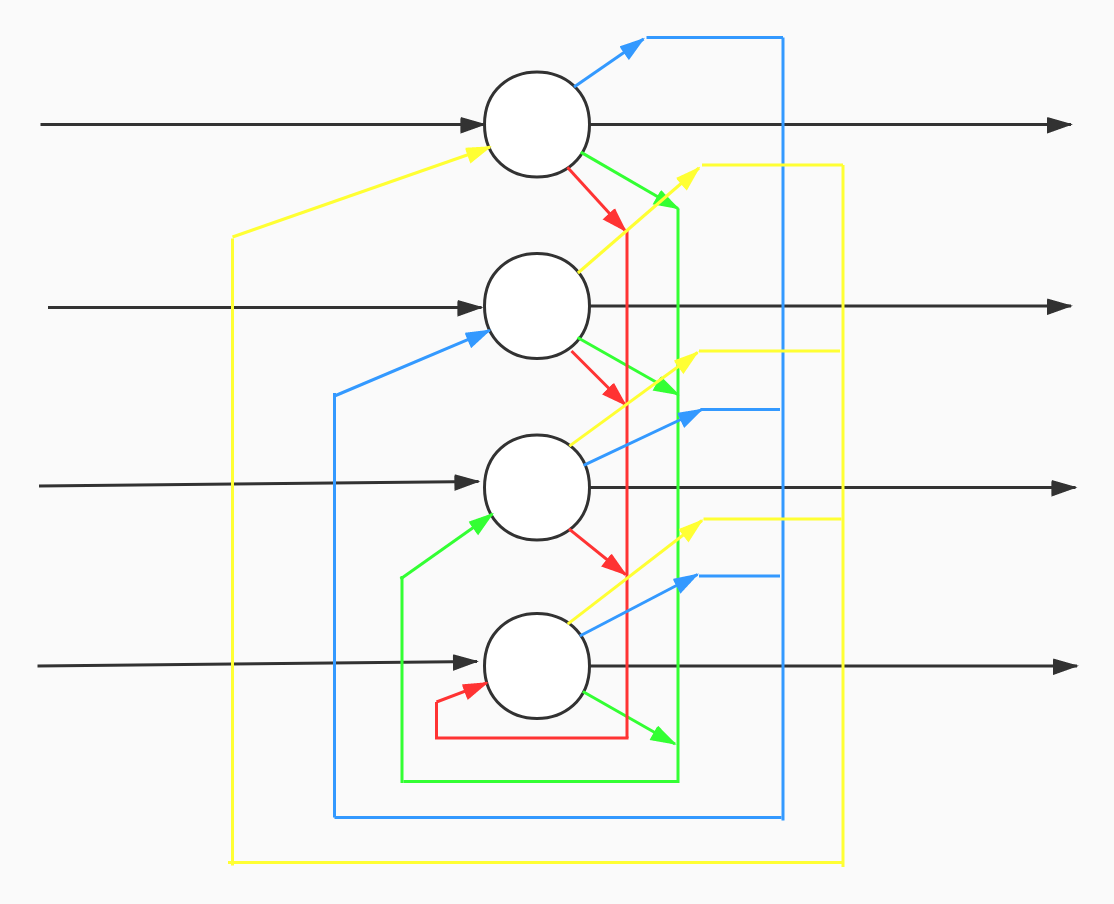
\includegraphics[width=13cm]{figure/Hopfield.jpg}
    \caption{Hopfield网络示意图}
    \label{fig-Hop}
\end{figure}
\par
1983年,Sejnowski和Hinton首次提出了“隐单元”的概念。玻尔兹曼机(Boltzmann Machine, BM)也以此被设计出来。
\begin{figure}[htbp]
    \centering
    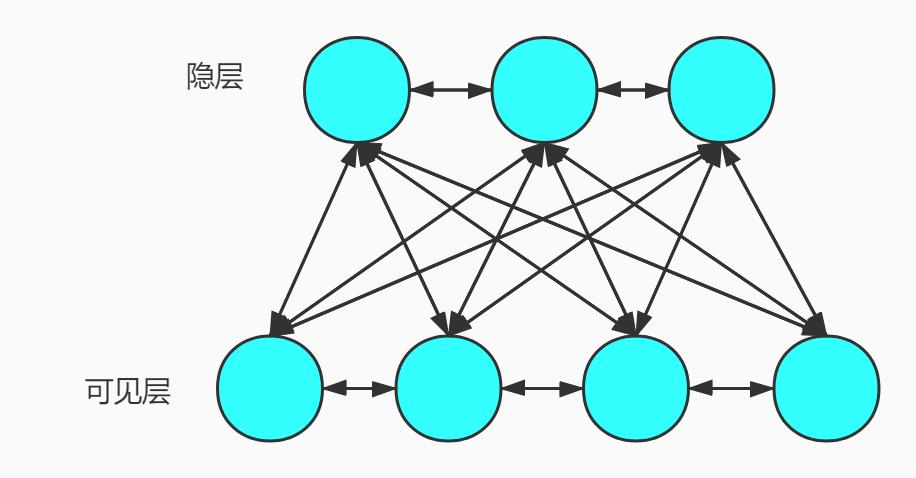
\includegraphics[width=13cm]{figure/BM.jpg}
    \caption{玻尔兹曼机结构示意图}
    \label{fig-BM}
\end{figure}
\par
Rumelhart与McCelland在1986年对反向传播算法进行了分析。其网络结构如下所示:
\begin{figure}[htbp]
    \centering
    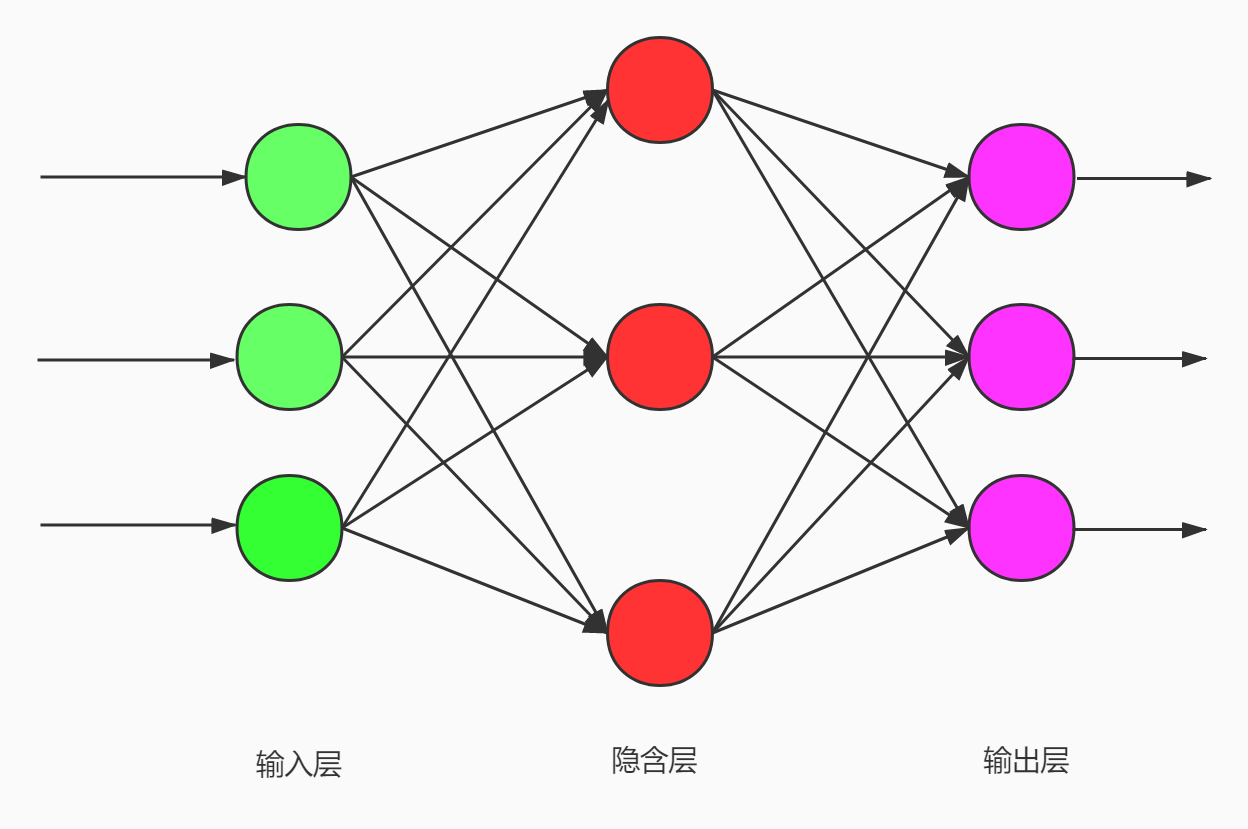
\includegraphics[width=13cm]{figure/BP.jpg}
    \caption{BP神经网络结构示意图}
    \label{fig-BP}
\end{figure}
BP除了隐含层,输入输出层的节点个数固定,而隐含层节点的选取可以使用经验公式确定即:
\begin{align}
    h = \sqrt{m+n} +a
\end{align}
隐含层节点数目为h,输入层节点数目记为m,输出节点数目记为n,a记为调节常数,$1 \le a \le 10$。\\
BP正向传播过程:\\
$\omega_{ij}$代表第i个节点与第j个节点的权值,$b_j$表示第j个节点的阈值。$x_j$表示第j个节点的输出值。
具体算法如下:
\begin{align}
    S_j  &= \sum_{i=0}^{m-1} \omega_{ij} x_i + b_j \\
    x_j &= f(S_j)
\end{align}
f代表激活函数,激活函数定义了该节点输入对应的输出,BP中选取线性或S型函数作为激活函数。
BP反向传播过程:
设输出层输出为$d_j$,则误差函数如下定义:
\begin{align}
    E(\omega, b) = \frac{1}{2} \sum_{j=1}^{n-1} (d_j-y_j)^2
\end{align}
Widrow-Hoff学习算法选取误差平方和下降最快的方向作为迭代方向,所以任意一个参数变化大小为:
\begin{align}
    \bigtriangleup \theta = - \eta \frac{\partial E_k}{\partial \theta} \label{tygz}%通用规则
\end{align}
其中,$\theta$ 代表BP中的任意一个参数,下面我们根据(\ref{tygz})来求解各个参数的更新公式:\\
假设激活函数为:\\
\begin{align}
    f(x) = \frac{A}{1+e^{-\frac{C}{B}}} \\
\end{align}
对激活函数求导:
\begin{align}
    f^{'}(x) &= \frac{Ae^{-\frac{C}{B}}}{B(1+e^{-\frac{C}{B}})^2} \\
    &=\frac{1}{AB} \cdot \frac{A}{1+e^{-\frac{C}{B}}} \cdot (A-\frac{A}{1+e^{-\frac{C}{B}}})\\
    &=\frac{f(x)[A-f(x)]}{AB}
\end{align}
则对于$\omega_{ij}$:
\begin{align}
    \frac{\partial E(\omega, b)}{\partial \omega_{ij}} &= \frac{1}{\partial \omega_{ij}} \cdot \frac{1}{2} \sum_{j=0}^{n-1} (d_j-y_j)^2 \\
    &=(d_j - y_j) \cdot \frac{\partial d_j}{\partial \omega_{ij}} \\
    &=(d_j-y_j) \cdot f^{'}(S_j) \cdot \frac{\partial S_j}{\partial \omega_{ij}} \\
    &=(d_j-y_j) \cdot \frac{f(S_j)[A-f(S_j)]}{AB} \cdot \frac{\partial S_j}{\partial \omega_{ij}} \\
    &=(d_j-y_j) \cdot \frac{f(S_j)[A-f(S_j)]}{AB} \cdot x_i \\
    &=\delta \cdot x_i
\end{align}
其中
\begin{align}
    \delta = (d_j-y_j) \cdot \frac{f(S_j)[A-f(S_j)]}{AB}
\end{align}
对于$b_j$也有:
\begin{align}
    \frac{\partial E(\omega, b)}{\partial b_j} = \delta_{ij}
\end{align}
下面介绍针对输入层和隐含层之间的权值与隐含层的阈值调整,下面设$\omega_{ki}$代表隐含层i节点与输入层k节点的权值:
\begin{align}
    \frac{\partial E(\omega , b)}{\partial \omega_{ki}} &=\frac{1}{\partial \omega_{ki}} \cdot \frac{1}{2} \sum_{j=0}^{n-1}(d_j-y_j)^2 \\
    &=\sum_{j=0}^{n-1} (d_j-y_j) \cdot f^{'}(S_j) \cdot \frac{\partial S_j}{\partial \omega_{ki}} \\
    &=\sum_{j=0}^{n-1} (d_j-y_j) \cdot f^{'}(S_j) \cdot \frac{\partial S_j}{\partial x_i} \cdot \frac{\partial x_i}{\partial S_i} \cdot \frac{\partial S_i}{\partial \omega_{ki}} \\
    &=\sum_{j=0}^{n-1} \delta_{ij} \cdot \omega_{ij} \cdot \frac{f(S_i)[A-f(S_i)]}{AB} \cdot x_k \\
    &=x_k \cdot \sum_{j=0}^{n-1} \delta_{ij} \cdot \omega_{ij} \cdot \frac{f(S_i)[A-f(S_i)]}{AB} \\
    &=\delta \cdot x_k
\end{align}
其中:
\begin{align}
    \delta = \sum_{j=0}^{n-1} \delta_{ij} \cdot \omega_{ij} \cdot \frac{f(S_i)[A-f(S_i)]}{AB}
\end{align}
所以根据上述公式,并结合梯度下降算法,隐含层与输出层之间的权值和阈值修改为:
\begin{align}
    \omega_{ij} &=\omega_{ij} - \eta_1 \cdot \frac{\partial E(\omega, b)}{\partial \omega_{ij}} = \omega_{ij} - \eta_1 \cdot \delta_{ij} \cdot x_i \\
    b_j &= b_j - \eta_2 \cdot \frac{\partial E(\omega, b)}{\partial b_j} = b_j - \eta_2 \cdot \delta_{ij}
\end{align}
同上,输入层与隐含层之间的权值和阈值修改为:
\begin{align}
    \omega_{ki} &= \omega_{ki} - \eta_1 \cdot \frac{\partial E(\omega ,b)}{\partial \omega_{ki}} = \omega_{ki} - \eta_1 \cdot \delta_{ki} \cdot x_k \\
    b_i &= b_i - \eta_2 \cdot \frac{\partial E(\omega, b)}{\partial b_i} = b_i - \eta_2 \cdot \delta_{ki}
\end{align}
由于本项目的实现主要是基于Hopfield,所以下一节我们将详细介绍Hopfield网络模型。
\section{Hopfield网络}
而本节主要介绍的是一种典型的反馈神经网络,Hopfield神经网络,该网络在1982年由美国物理学家Hopfield创立,并由1984年实现了该网络的硬件电路设计,
Hopfield的论文中描述了该网络可以应用于组合优化问题,比如组合优化的经典问题TSP问题,所以Hopfield与Tank使用Hopfield网络求解了30个城市的TSP问题,1987年贝尔实验室在Hopfield的基础上研制出了神经网络的芯片,
Hopfield首次在神经网络领域引入了“能量函数”的概念,并且证明了网络的稳定性,Hopfield网络是神经网络领域一个里程碑式的发现。
\subsection{Hopfield网络模型}
Hopfield模型被划分为连续性(CHNN)与离散型(DHNN),本项目用的是连续性神经网络,其中连续型可以去解决组合优化问题,
离散型常用于处理联想记忆,如文字识别等。
%\begin{figure}[htbp]
%    \centering
%    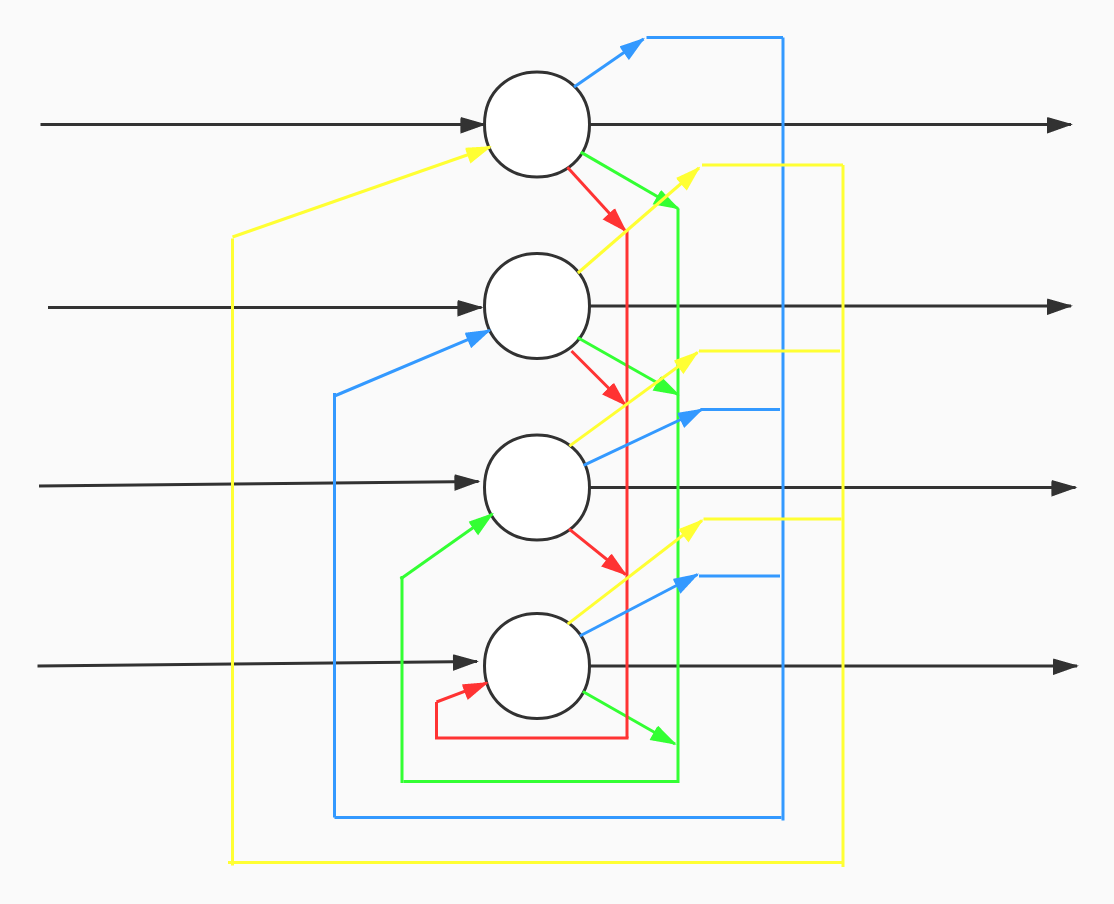
\includegraphics[width=13cm]{figure/Hopfield.jpg}
%    \caption{Hopfield网络示意图}
%    \label{fig-Hop}
%\end{figure}
\par
(1)离散型:
\newline
离散Hopfield(Discrete Hopfield Network, DHNN)的结构是单层的反馈网络。Hopfield在论文中最早提出的是二值神经网络,即神经元的输出只有-1,1两个值,
所以又被称为离散型Hopfield网络,在输出的0,1中1表示激活,-1表示抑制。
\begin{figure}[htbp]
    \centering
    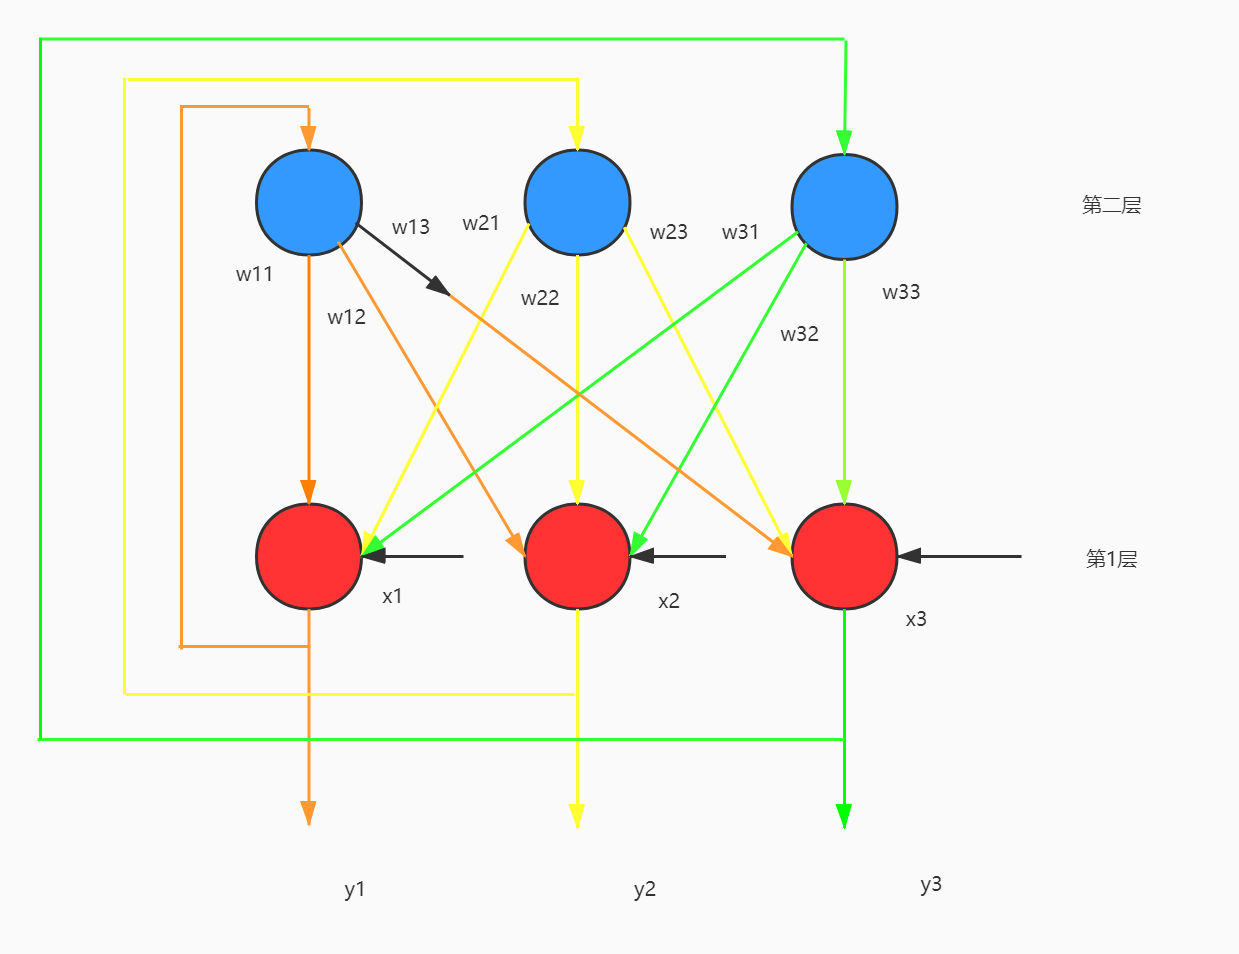
\includegraphics[width=13cm]{figure/DHNN.jpg}
    \caption{离散型Hopfield神经网络}
    \label{fig-DHNN}
\end{figure}
在图(\ref{fig-DHNN})中,神经元一共在0层和1层中,其中0层没有计算的功能即他没有履行实际神经元的职能,所以它仅仅作为网络的输入看待;
下面列出神经元的计算公式。
\begin{align}
    u_i = \sum_i \omega_{ij} y_i + x_i
\end{align}
其中上式中的$x_i$为输入。其中$y_i$为:
\begin{equation}
    y_i=
    \begin{cases}
        +1,\quad u_j \ge \theta_j \\
        -1,\quad u_j < \theta_j
    \end{cases}
\end{equation}
输出层是一个n维向量,假设该向量在t时刻的定义为:
\begin{align}
    Y(t) = [y_1(t), y_2(t), \cdots, y_n(t)]^T
\end{align}
所以输出层向量的状态一共有$2^n$中,所以我们可以认为网络的状态也有$2^n$种,
而输出状态之间的迭代公式如下所示:
\begin{equation}
y_j(t+1)=f[u_j(t)]=
    \begin{cases} 
        +1,\quad u_j(t) \ge 0 \\
        -1,\quad u_j(t) < 0 
    \end{cases}
    \label{scdd}%输出迭代
\end{equation}
\begin{align}
    u_j(t) = \sum_{i=1}^n \omega_{ij} y_i(t) + x_j - \theta_j \label{srdd} %输入迭代
\end{align}
其中$y_i(t)$ 表示输出层第$i$个节点在第t个时刻的状态,从上式我们可以看出如果$i=j$时$\omega_{ij} = 0$ 则新状态的输入不会由旧状态的输出影响,我们称这种网络为无自反馈网络;
反之如果在$i =j $时$\omega_{ij} \ne 0$,则旧状态的输出会影响新状态的输入,所以我们称这种网络为有自反馈的网络。\\
(2)连续性:
\par
连续性Hopfield(Continuous Hopfield Neural Network, CHNN),CHNN神经网络与DHNN神经网络的网络结构相似,二者的不同点在于它传递的函数
不是存在间断的函数,而是连续函数。
\begin{figure}[htbp]
    \centering
    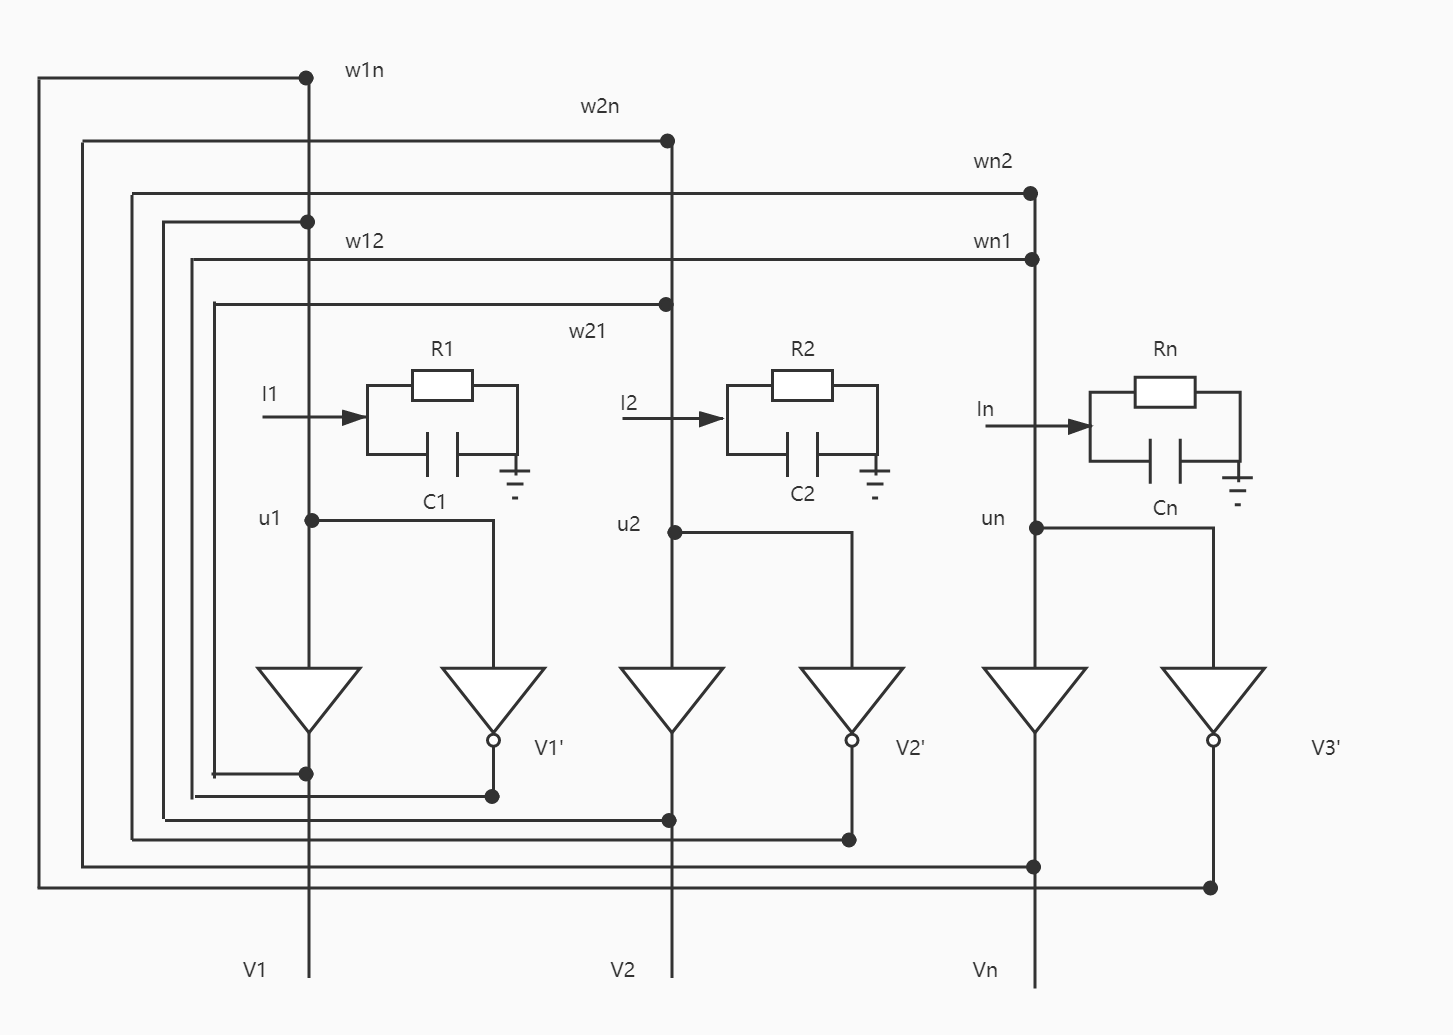
\includegraphics[width=13cm]{figure/CHNN.jpg}
    \caption{连续性Hopfield神经网络}
    \label{fig-CHNN}
\end{figure}
在硬件上是由简单的线路连接来实现,其神经元的输出时随着时间变化而变化的。为了模拟神经元$S$型的函数关系,则采用饱和非线性运算放大器来模拟如下图(\ref{fig-ysfdq})所示,且该函数关系为:
\begin{figure}[htbp]
    \centering
    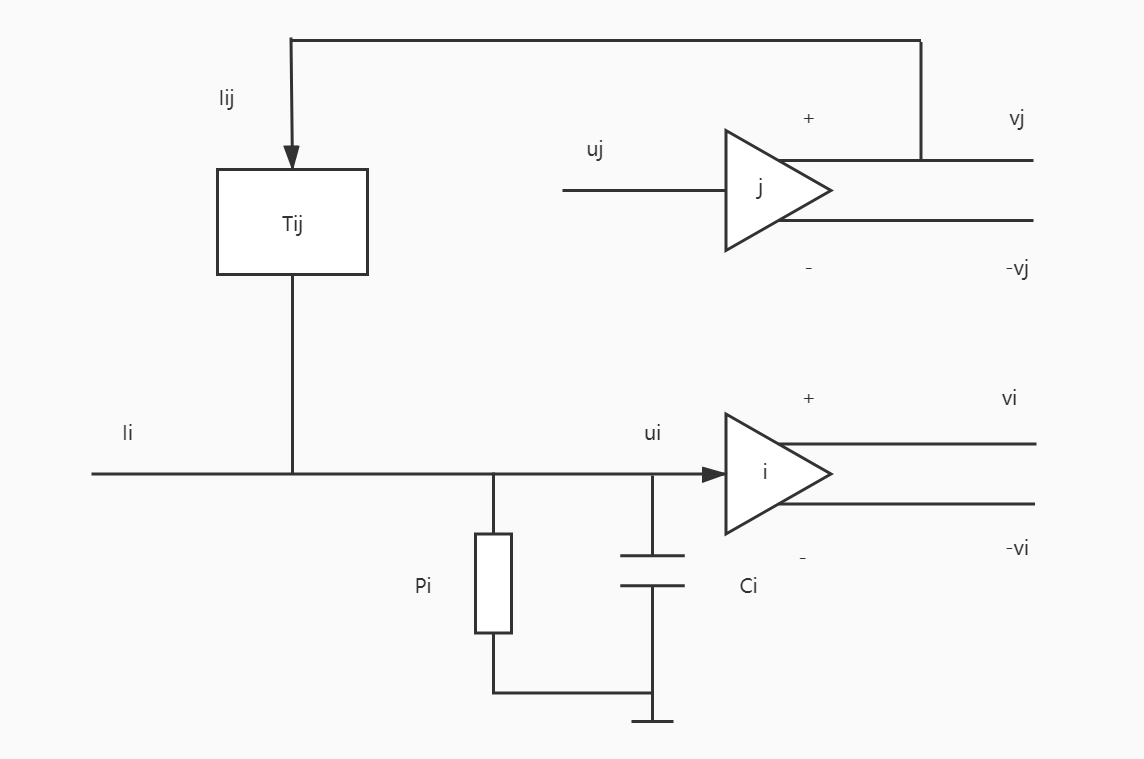
\includegraphics[width=13cm]{figure/xhfdq.jpg}
    \caption{饱和非线性运算放大器}
    \label{fig-ysfdq}
\end{figure}
\begin{align}
    v_i = f_i(u_i)
\end{align}
对于$N$个节点的CHNN神经元的迭代变化规则使用微分方程来规定即:
\begin{numcases}{}
    C_i \frac{du_i}{dt} = \sum_{j=1}^N T_{ij}v_j-\frac{u_i}{R_i} + I_i \\
    v_i = f_i(u_i) \\
    i = 1,2,3,\cdots, N
    \label{wffc}%微分方程
\end{numcases}
能量函数的定义为:
\begin{align}
    E = -\frac{1}{2} \sum_{i=1}^N \sum_{\substack{j=1 \\ j \ne i}}^N T_{ij} v_i v_j -\sum_{i=1}^N v_i I_i + \sum_{i=1}^N \frac{1}{R_i} \int_0^{v_i} f^(-1)(v)dv 
\end{align}
虽然CHNN的能量函数在表达形式上与物流意义上的能量函数一致,但是它的实际意义时为了表示网络的状态的变化。
\subsection{Hopfield网络的学习算法}
Hopfield的工作方式分为异步与同步,其中异步工作方式也叫串行工作方式,即在任意时刻只有一个神经元进行状态更新,其状态更新规则
遵循(\ref{scdd})与(\ref{srdd})二式。而同步工作方式又被称为并行工作方式,即在某一时刻全部或部分神经元的状态进行更新。
下面说明离散型与连续性Hopfield网络的学习规则。\\
(1)离散型:\\
1.外积法:\\
假设其样本数据为$\{t^1,t^2,t^3,\cdots, t^N\}$其中任意元素的状态为1,-1,学习规则如下:
\begin{align}
    W = \sum_{k=1}^N [t^k(t^k)^T-I] \label{wjgz} %外积规则
\end{align}
该规则被称为“外积规则”。下面我们简单描述其建立Hopfield神经网络的步骤。\\
\par
$Step \quad 1$: 将样本数据根据(\ref{wjgz})计算权系数矩阵。
\par
$Step \quad 2$: 初始化网络输出值,并规定网络的迭代次数。
\par
$Step \quad 3$: 迭代公式如下所示:
\begin{align}
    y_i(k+1) = f(\sum_{j=1}^N \omega_{ij} y_j)
\end{align}
\par
$Step \quad 4$: 迭代中止条件定为网络状态不变或网络迭代到达最大次数,如果不满足终止条件则返回Step 3。\\
2.正交化法:\\
算法步骤如下:\\
\par
$Step \quad 1: \quad $初始化N个输入设为$t = \{t^2,t^2,\cdots, t^(N-1) ,t^N\}$,参数$\tau,h$。
\par
$Step \quad 2: \quad $计算$=\{t^2-t^N,t^2-t^N,\cdots,t^(N-1)-t^N\}$。
\par
$Step \quad 3: \quad $奇异值分解$A=USV^T$,并求$K = rank(A)$。
\par
$Step \quad 4: \quad $由$U^p = \{U^1,U^2,U3,\cdots,U^k\}$与$u^m = \{u^(K+1),u^(K+2),\cdots, u^N\}$求出$T^p = \sum_{i=1}^k u^i (u^i)^T, T^m = \sum_{i=K+1}^N u^i (u^i)^T$。
\par
$Step \quad 5: \quad $求$W^t = T^p-\tau \times T^m, b^t = t^N-W^t \times t^N$。
\par
$Step \quad 6: \quad $求$W = exp(h \times W^t)$。
\par
$Step \quad 7: \quad $求$b = U \times \left[\begin{array}{cc}
    C_{1} \times I(K) & 0(K, N-K) \\
    0(N-K, K) & C_{2} \times I(N-K)
    \end{array}\right] \times U^T \times b^t $其中$C_1 = exp(h) - 1, C_2 = -[exp(-\tau \times h) - 1]/\tau$。\\
(2)连续型:
连续型Hopfield神经网络解决优化问题主要分为以下步骤:
\begin{figure}[htbp]
    \centering
    
\includegraphics[width=13cm]{figure/Hoplct.jpg}%hop流程图
    \caption{Hopfield解决优化计算的步骤}
    \label{fig-Hoplct}
\end{figure}







